% ============================================================
% 40-bezier-code-analysis.tex
% Compile with:  pdflatex -shell-escape 40-bezier-code-analysis.tex
% Run twice for table of contents.
% ============================================================

\documentclass[12pt, a4paper]{article}

\usepackage[T1]{fontenc}
\usepackage[utf8]{inputenc}
\usepackage{lmodern}
\usepackage[top=2.5cm, bottom=2.5cm, left=2.8cm, right=2.8cm]{geometry}
\usepackage[dvipsnames]{xcolor}

\definecolor{codebg}{RGB}{248,248,248}
\definecolor{rulecolor}{RGB}{180,180,180}
\definecolor{examplebg}{RGB}{240,248,255}
\definecolor{examplerule}{RGB}{100,149,237}
\definecolor{notebg}{RGB}{255,250,230}
\definecolor{noterule}{RGB}{210,180,50}
\definecolor{diffbg}{RGB}{240,255,240}
\definecolor{diffrule}{RGB}{80,160,80}
\definecolor{warnbg}{RGB}{255,245,245}
\definecolor{warnrule}{RGB}{200,80,80}

\usepackage{minted}
\setminted[julia]{
  bgcolor=codebg, frame=leftline, framerule=1.5pt,
  rulecolor=rulecolor, linenos=false, fontsize=\small,
  breaklines=true, tabsize=4, style=friendly,
}

\usepackage{amsmath}
\usepackage{amssymb}
\usepackage{tikz}
\usetikzlibrary{shapes.geometric, arrows.meta, positioning,
                matrix, fit, backgrounds, decorations.pathreplacing}
\usepackage{mdframed}
\usepackage{graphicx}
\usepackage{float}

\newmdenv[backgroundcolor=examplebg, linecolor=examplerule,
  linewidth=1.5pt, leftline=true, rightline=false,
  topline=false, bottomline=false,
  innerleftmargin=10pt, innerrightmargin=8pt,
  innertopmargin=6pt, innerbottommargin=6pt,
  skipabove=6pt, skipbelow=4pt]{examplebox}

\newmdenv[backgroundcolor=notebg, linecolor=noterule,
  linewidth=1.5pt, leftline=true, rightline=false,
  topline=false, bottomline=false,
  innerleftmargin=10pt, innerrightmargin=8pt,
  innertopmargin=6pt, innerbottommargin=6pt,
  skipabove=6pt, skipbelow=4pt]{notebox}

\newmdenv[backgroundcolor=diffbg, linecolor=diffrule,
  linewidth=1.5pt, leftline=true, rightline=false,
  topline=false, bottomline=false,
  innerleftmargin=10pt, innerrightmargin=8pt,
  innertopmargin=6pt, innerbottommargin=6pt,
  skipabove=6pt, skipbelow=4pt]{insightbox}

\newmdenv[backgroundcolor=warnbg, linecolor=warnrule,
  linewidth=1.5pt, leftline=true, rightline=false,
  topline=false, bottomline=false,
  innerleftmargin=10pt, innerrightmargin=8pt,
  innertopmargin=6pt, innerbottommargin=6pt,
  skipabove=6pt, skipbelow=4pt]{tradebox}

\usepackage[colorlinks=true, linkcolor=black, urlcolor=MidnightBlue]{hyperref}
\usepackage{booktabs}
\usepackage{needspace}
\usepackage{parskip}
\usepackage{titlesec}
\usepackage{fancyhdr}
\usepackage{datetime2}
\usepackage{multirow}
\usepackage{array}
\usepackage{colortbl}

\titleformat{\section}
  {\large\bfseries\color{MidnightBlue}}{\thesection.}{0.6em}{}
  [\vspace{-4pt}\rule{\linewidth}{0.4pt}]
\titleformat{\subsection}
  {\normalsize\bfseries\color{BrickRed}}{\thesubsection.}{0.5em}{}
\titleformat{\subsubsection}
  {\normalsize\bfseries}{\thesubsubsection.}{0.5em}{}

\pagestyle{fancy}
\fancyhf{}
\rhead{\textcolor{gray}{\small 40-bezier-code-analysis}}
\lhead{\textcolor{gray}{\small B\'ezier Series --- Code Analysis}}
\cfoot{\thepage}
\renewcommand{\headrulewidth}{0.3pt}

\newcommand{\cd}[1]{\texttt{#1}}
\newcommand{\script}[1]{\textbf{\texttt{#1}}}

\title{%
  \vspace{1cm}
  {\LARGE\bfseries B\'ezier Curve Series}\\[0.4em]
  {\large Code Analysis and Design Review}\\[0.4em]
  {\normalsize Scripts 01--35: Architecture, Patterns,
   Trade-offs, and Julia Lessons}
}
\author{E.R.\ Nurwijayadi}
\date{\DTMtoday}

\begin{document}

\maketitle
\thispagestyle{empty}

\begin{center}
\textit{Directed and curated by E.R.\ Nurwijayadi.
Code and explanations AI-generated.}
\end{center}

\begin{center}
\begin{minipage}{0.85\textwidth}
\small
This document steps back from individual script explanations
and analyses the series as a whole.
It covers the architectural progression across all 15 scripts,
recurring code patterns, deliberate design decisions and
their trade-offs, Julia-specific idioms introduced along the
way, and the curvature thread that connects the later scripts.
\end{minipage}
\end{center}

\vspace{1em}\hrule\vspace{1.5em}
\tableofcontents
\newpage


% =============================================================
\needspace{8\baselineskip}
\section{Part 1: Architecture of the Series}
% =============================================================

\subsection{The Three-Axis Progression}

The 15 scripts are not random --- they form a deliberate
path through a three-dimensional design space.
Each axis is varied independently, so the reader can
isolate one change at a time.

\bigskip

\begin{center}
\begin{tikzpicture}[font=\small]
  \draw[-Stealth, thick, MidnightBlue]
    (0,0) -- (10,0) node[right]{\textbf{Computation method}};
  \draw[-Stealth, thick, BrickRed]
    (0,0) -- (0,5)  node[above]{\textbf{Output type}};
  \draw[-Stealth, thick, OliveGreen]
    (0,0) -- (-2.5,-2.0) node[below left]{\textbf{Arithmetic}};

  % Computation axis labels
  \node[MidnightBlue, below] at (2,0)   {\footnotesize Bernstein};
  \node[MidnightBlue, below] at (4.5,0) {\footnotesize Matrix};
  \node[MidnightBlue, below] at (7,0)   {\footnotesize Generic};
  \node[MidnightBlue, below] at (9.5,0) {\footnotesize Interactive};

  % Output axis labels
  \node[BrickRed, right] at (0,1.2) {\footnotesize Text};
  \node[BrickRed, right] at (0,2.4) {\footnotesize 2-D plot};
  \node[BrickRed, right] at (0,3.6) {\footnotesize 3-D static};
  \node[BrickRed, right] at (0,4.8) {\footnotesize Interactive};

  % Arithmetic axis labels
  \node[OliveGreen, left] at (-0.8,-0.65) {\footnotesize Float64};
  \node[OliveGreen, left] at (-1.6,-1.3)  {\footnotesize Rational};
  \node[OliveGreen, left] at (-2.4,-1.95) {\footnotesize Symbolic};
\end{tikzpicture}
\end{center}

\bigskip

\subsection{Script Map: All 15 Scripts on Three Axes}

\begin{center}
\renewcommand{\arraystretch}{1.25}
\begin{tabular}{llllll}
\toprule
Script & Computation & Arithmetic & Output & New concept \\
\midrule
\rowcolor{examplebg}
01 & Bernstein (hand) & Float64 & Text & \cd{Poly} type, operator overloading \\
02 & Bernstein & Rational & Text & Symbolics.jl, \cd{@variables} \\
\rowcolor{examplebg}
03 & Matrix (pedagogical) & Float64 & Text & $U \cdot M \cdot G$, derive\_M \\
04 & Matrix (straight) & Float64 & Text & Section-based output \\
\rowcolor{examplebg}
05 & Matrix & Rational & Text & \cd{fmt\_poly} bridging types \\
\midrule
11p & Bernstein & Float64 & 2-D plot & Plots.jl, \cd{hcat+splat+transpose} \\
\rowcolor{examplebg}
11m & Bernstein & Float64 & 2-D plot & CairoMakie, Figure/Axis split \\
12p & De Casteljau & Float64 & 2-D plot & \cd{lerp}, named tuple return \\
\rowcolor{examplebg}
12m & De Casteljau & Float64 & 2-D plot & \cd{titlegap}, no \cd{label} = hidden \\
\midrule
21 & Bernstein & Float64 & 3-D static & \cd{Axis3}, elevation/azimuth \\
\rowcolor{examplebg}
22 & De Casteljau & Float64 & 3-D static & \cd{getfield}, NaN dummy lines \\
31 & Generic Bernstein & Float64 & 2-D/3-D & \cd{is\_3d} branch, \cd{while} DC \\
\rowcolor{examplebg}
32 & Generic Symbolic & Mixed & 2-D/3-D & \cd{build\_symbolic\_poly} \\
34 & Generic + Curvature & Float64 & 2-D/3-D & \cd{d1\_pts}/\cd{d2\_pts}, \cd{draw\_comb!} \\
\rowcolor{examplebg}
35 & Interactive & Float64 & UI & \cd{Observable}, \cd{Toggle}, \cd{Textbox} \\
\bottomrule
\end{tabular}
\end{center}

\subsection{How the Series Teaches}

\begin{insightbox}
\textbf{Each script introduces exactly one new idea.}

Scripts 01--05 vary only the \emph{arithmetic} (Float64
vs Rational) and the \emph{method} (Bernstein vs matrix),
keeping the output as plain terminal text.
This isolates the mathematics from all plotting concerns.

Scripts 11--12 introduce plotting for the first time,
but use the simplest possible curve (quadratic 2-D)
so the new plotting API is not competing with new math.

Scripts 21--22 add 3-D, but reuse the quartic curve
already understood from scripts 01--05.

Scripts 31--35 generalise everything, stacking interactivity
on top of the generic architecture one layer at a time.

A beginner can follow each step without being overwhelmed
because the foundation is always already familiar.
\end{insightbox}


% =============================================================
\needspace{8\baselineskip}
\section{Part 2: Recurring Code Patterns}
% =============================================================

\subsection{The Universal Curve Matrix Builder}

The same three-step idiom appears in \emph{every} plotting
script from 11 onward:

\begin{minted}{julia}
hcat([f(bz, u) for u in u_vals]...)'
\end{minted}

\begin{center}
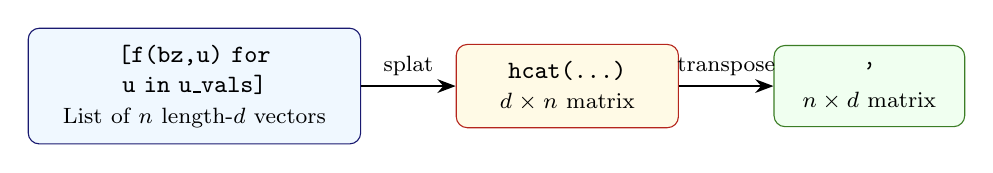
\begin{tikzpicture}[font=\small, node distance=0.3cm]
  \node[draw=MidnightBlue, rounded corners, fill=examplebg,
        inner sep=6pt, text width=3.8cm, align=center] (comp)
    {\cd{[f(bz,u) for u in u\_vals]}\\
     \footnotesize List of $n$ length-$d$ vectors};
  \node[draw=BrickRed, rounded corners, fill=notebg,
        inner sep=6pt, text width=2.4cm, align=center,
        right=1.2cm of comp] (hcat)
    {\cd{hcat(\ldots)}\\
     \footnotesize $d \times n$ matrix};
  \node[draw=OliveGreen, rounded corners, fill=diffbg,
        inner sep=6pt, text width=2.0cm, align=center,
        right=1.2cm of hcat] (trans)
    {\cd{'}\\
     \footnotesize $n \times d$ matrix};
  \draw[-Stealth,thick] (comp) -- node[above]{\footnotesize splat}
    (hcat);
  \draw[-Stealth,thick] (hcat) -- node[above]{\footnotesize transpose}
    (trans);
\end{tikzpicture}
\end{center}

\begin{center}
\begin{tabular}{lll}
\toprule
Script & Function & Result shape \\
\midrule
11 & \cd{curve(bz)} & $200 \times 2$ \\
12 & \cd{dc\_curve(dc)} & $200 \times 2$ \\
21 & \cd{bq\_curve(bz)} & $300 \times 3$ \\
31 & \cd{bz\_curve(bz)} & $300 \times \text{dim}$ \\
34 & \cd{bz\_curve(pts)} & $300 \times \text{dim}$ \\
35 & \cd{bz\_curve(pts)} & $300 \times \text{dim}$ \\
\bottomrule
\end{tabular}
\end{center}

The pattern is identical in every script.
Once a reader understands it in script~11, they
recognise it immediately in all subsequent scripts.

\needspace{5\baselineskip}
\subsection{The \texttt{CASE} Switch Pattern}

\begin{minted}{julia}
const CASE = 2   # only change this line

const CASE_DATA = Dict(
    1 => ( points = ..., output = "...", ),
    2 => ( points = ..., output = "...", ),
)

function main()
    data = CASE_DATA[CASE]
    ...
end
\end{minted}

This pattern appears in scripts 01--05, 31, 32, 34.
It separates the \emph{configuration} (what case to run)
from the \emph{logic} (how to run it).
The single line \cd{const CASE = N} is the only line
a user needs to change.

\begin{center}
\begin{tabular}{ll}
\toprule
What varies between cases & What stays constant \\
\midrule
Control point matrix (shape and values) &
  All math functions \\
Number of dimensions (2 or 3) &
  All drawing functions \\
Output filename &
  The \cd{CASE} switch mechanism \\
$u$ highlight values &
  \cd{main()} structure \\
\bottomrule
\end{tabular}
\end{center}

\needspace{5\baselineskip}
\subsection{The \texttt{is\_3d} Branch Pattern}

Scripts 31, 32, 34, 35 all contain blocks of the form:

\begin{minted}{julia}
if is_3d
    lines!(ax, xs, ys, zs, ...)
else
    lines!(ax, xs, ys, ...)
end
\end{minted}

This appears for every drawing call: \cd{lines!},
\cd{scatter!}, \cd{text!}, axis creation, limit setting.
The duplication is deliberate --- it keeps each branch
self-contained and easy to read, even though it is verbose.

An alternative would be to pass coordinates as a tuple
and splat them: \cd{lines!(ax, coords...)}.
This would halve the number of lines but make each line
harder to read.
The series chose readability over compactness.

\needspace{5\baselineskip}
\subsection{The \texttt{while} De Casteljau Loop}

\begin{minted}{julia}
levels  = Matrix{Float64}[copy(pts)]
current = copy(pts)
while size(current, 1) > 1
    n       = size(current, 1)
    current = vcat([((1-u).*current[j,:] .+ u.*current[j+1,:])' for j in 1:n-1]...)
    push!(levels, current)
end
\end{minted}

This exact pattern appears in scripts 31, 32, 34, 35.
It replaces the explicit level-by-level functions from
scripts 12 and 22 (\cd{reduce\_level} called four times).
The \cd{while} version works for any degree automatically.

\begin{center}
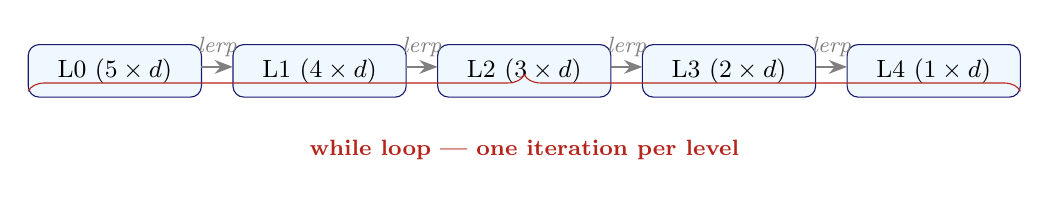
\begin{tikzpicture}[font=\small]
  \foreach \n/\label in
    {5/L0 ($5\times d$), 4/L1 ($4\times d$),
     3/L2 ($3\times d$), 2/L3 ($2\times d$), 1/L4 ($1\times d$)} {
    \node[draw=MidnightBlue, fill=examplebg, rounded corners,
          inner sep=5pt, minimum width=2.2cm]
      at ({(\n-5)*(-2.6)}, 0) {\label};
  }
  \foreach \from/\to in {5/4, 4/3, 3/2, 2/1} {
    \draw[-Stealth, thick, gray]
      ({(\from-5)*(-2.6)+1.1}, 0.05) --
      node[above, font=\footnotesize\itshape]{lerp} 
      ({(\to-5)*(-2.6)-1.1}, 0.05);
  }
  \draw[decorate, decoration={brace, amplitude=6pt, raise=4pt},
        BrickRed]
    ({(5-5)*(-2.6)-1.1}, -0.4) -- ({(1-5)*(-2.6)+1.1}, -0.4)
    node[midway, below=10pt, BrickRed, font=\footnotesize\bfseries]
    {while loop --- one iteration per level};
\end{tikzpicture}
\end{center}

\needspace{5\baselineskip}
\subsection{Colour-with-Alpha Tuples}

Makie accepts colours as \cd{(name, alpha)} pairs.
This pattern appears in every Makie script from script~22 onward:

\begin{center}
\begin{tabular}{lll}
\toprule
Usage & Code & Meaning \\
\midrule
Construction line & \cd{(col, 0.75)} & 75\% opacity \\
Connector line & \cd{(col, 0.35)} & 35\% --- very faint \\
Comb spike & \cd{(:slategray, 0.5)} & 50\% \\
Comb envelope & \cd{(:slategray, 0.4)} & 40\% \\
Legend frame & \cd{(:black, 0.3)} & 30\% \\
Legend background & \cd{(:white, 0.8)} & 80\% \\
\bottomrule
\end{tabular}
\end{center}

The pattern lets the reader layer visual information:
full-opacity elements (curve, markers) are foreground;
semi-transparent elements (construction lines, comb) are background.

\needspace{5\baselineskip}
\subsection{Legend Control: Three Strategies}

Across the scripts, three different strategies are used
to control which elements appear in the legend:

\begin{center}
\begin{tabular}{lp{3.5cm}p{4.5cm}}
\toprule
Strategy & Code & When used \\
\midrule
Include & \cd{label = "name"} &
  Main elements: curve, polygon, highlighted points \\
Exclude (Plots.jl) & \cd{label = false} &
  Auxiliary scatter dots (De Casteljau levels) \\
Exclude (Makie) & (omit \cd{label}) &
  Same effect in Makie --- no keyword = no entry \\
Placeholder & \cd{label = ""} &
  Script 31: dot-only legend entries for level colours \\
NaN dummy & \cd{lines!([NaN],[NaN],[NaN], label=lbl)} &
  Script 22: style entries (solid/dashed/dotted) \\
\bottomrule
\end{tabular}
\end{center}

\begin{insightbox}
\textbf{NaN as an invisible marker.}
The NaN dummy line pattern (script~22) is a professional
trick used in real scientific plotting code.
It lets you add a legend entry that explains a visual
convention (line style, colour) without drawing anything
visible in the plot area.
\end{insightbox}


% =============================================================
\needspace{8\baselineskip}
\section{Part 3: Design Decisions and Trade-offs}
% =============================================================

\subsection{Struct Design: How It Evolved}

The struct holding control points changed four times across
the series, each time for a clear reason:

\begin{center}
\renewcommand{\arraystretch}{1.3}
\begin{tabular}{lp{3.0cm}p{3.0cm}p{3.5cm}}
\toprule
Scripts & Struct & Fields & Why \\
\midrule
11--12 &
  \cd{BezierQuadratic} &
  \cd{p0, p1, p2 ::Vector} &
  3 named fields are readable; small fixed degree \\[4pt]
21 &
  \cd{BezierQuartic} &
  \cd{points ::Matrix} &
  5 fields would be clutter; matrix is cleaner \\[4pt]
31--33 &
  \cd{BezierCurve} &
  \cd{points, n, degree, dim} &
  Generic: infers all metadata from matrix shape \\[4pt]
34--35 &
  \cd{BezierCurve} (extended) &
  + \cd{d1\_pts, d2\_pts} &
  Curvature needs pre-computed derivative control points \\
\bottomrule
\end{tabular}
\end{center}

\begin{tradebox}
\textbf{Named fields vs matrix field:}

\cd{BezierQuadratic} with \cd{p0, p1, p2} is readable
in the point function:
\begin{minted}{julia}
b0 .* bz.p0 .+ b1 .* bz.p1 .+ b2 .* bz.p2
\end{minted}

But for 5 points it becomes:
\begin{minted}{julia}
b0.*bz.p0 .+ b1.*bz.p1 .+ b2.*bz.p2 .+ b3.*bz.p3 .+ b4.*bz.p4
\end{minted}

The generic \cd{sum(bernstein(...) .* bz.points[i,:] for i ...)}
is shorter and works for any degree.
The trade-off: named fields are self-documenting;
indexed access is compact but requires knowing the convention.
\end{tradebox}

\needspace{5\baselineskip}
\subsection{Arithmetic Choice: Float64 vs Rational\{Int\}}

\begin{center}
\begin{tabular}{p{1.5cm}p{4.5cm}p{5cm}}
\toprule
Type & Strengths & Weaknesses \\
\midrule
\cd{Float64} &
  Fast; compatible with all plotting; natural for most users &
  Rounding error accumulates; \cd{rationalize()} needed
  to display fractions \\[6pt]
\cd{Rational\{Int\}} &
  Exact; fractions display naturally as \cd{269//256};
  no rounding error &
  Slower; denominators grow; needs conversion to Float64
  for display \\
\bottomrule
\end{tabular}
\end{center}

Scripts 02 and 05 use \cd{Rational\{Int\}} to demonstrate
that the exact fractions computed algebraically
(scripts 01--05) genuinely match the plotted values.
The rest of the series uses \cd{Float64} because
plotting coordinates are inherently approximate.

\needspace{5\baselineskip}
\subsection{CairoMakie vs GLMakie}

\begin{center}
\begin{tabular}{lll}
\toprule
Backend & Used in & Reason \\
\midrule
\cd{CairoMakie} & Scripts 11m, 12m, 21, 22 &
  Static PNG output; no display server needed \\
\cd{GLMakie} & Scripts 31, 32, 34, 35 &
  Interactive window; 3-D rotation with mouse \\
\bottomrule
\end{tabular}
\end{center}

The switch from CairoMakie to GLMakie at script~31
coincides with the introduction of the generic
\cd{is\_3d} architecture.
Once a script could produce either a 2-D or 3-D plot,
interactivity became more valuable --- and GLMakie's
mouse-driven 3-D rotation makes the quartic 3-D case
much easier to explore.

\needspace{5\baselineskip}
\subsection{Named Functions vs Inline: The De Casteljau Progression}

\begin{center}
\renewcommand{\arraystretch}{1.3}
\begin{tabular}{lp{4cm}p{5.5cm}}
\toprule
Scripts & Approach & Trade-off \\
\midrule
12 &
  \cd{lerp} + \cd{steps()} named tuple &
  Clean, readable, but fixed at quadratic \\
22 &
  \cd{lerp3} + \cd{reduce\_level} + \cd{dc\_steps} &
  More general (any level count) but still fixed degree \\
31--35 &
  Inline \cd{while} loop, no separate functions &
  Maximally general; self-contained; harder to unit-test \\
\bottomrule
\end{tabular}
\end{center}

The progression shows a deliberate move from
\emph{pedagogical clarity} (named function per concept)
toward \emph{engineering compactness} (one generic loop).
Both have value --- the individual function approach
is better for teaching; the loop is better for production.

\needspace{5\baselineskip}
\subsection{Symbolic vs Numeric Evaluation}

Scripts 31 and 32 produce identical plots from visually
identical code.
The difference is entirely in how \cd{bz\_point} works:

\begin{center}
\begin{tabular}{lp{4.5cm}p{4.5cm}}
\toprule
Script & Method & Suitable when \\
\midrule
31 &
  Direct Bernstein: $\sum B(n,i,u) \cdot P_i$ per call &
  You want speed and simplicity \\[4pt]
32 &
  Build polynomial once; substitute $u$ for each evaluation &
  You want to inspect, differentiate, or print
  the polynomial itself \\
\bottomrule
\end{tabular}
\end{center}

Script~32's \cd{main()} prints the expanded polynomials
to the terminal before drawing --- something script~31
cannot do.
This connects the plotting scripts back to the algebraic
results of scripts~01--05, closing a loop in the series.


% =============================================================
\needspace{8\baselineskip}
\section{Part 4: Julia-Specific Lessons}
% =============================================================

\subsection{Lesson Map: Which Script Teaches What}

\begin{center}
\renewcommand{\arraystretch}{1.3}
\begin{tabular}{lp{5cm}l}
\toprule
Julia concept & What it is & First seen \\
\midrule
Multiple dispatch &
  Same function name, different behaviour by type &
  Script~01 (\cd{fmt\_rat}) \\
Struct + outer constructor &
  Derived fields computed in constructor &
  Scripts~01, 11 \\
Broadcast (\cd{.* .+}) &
  Element-wise operation on any array shape &
  Script~11 \\
Named tuple return &
  \cd{return (field1=v1, field2=v2)} &
  Script~12 \\
\cd{sum(generator; init=)} &
  Accumulate a computed series with a type-providing seed &
  Script~05 \\
\cd{Union\{T, Nothing\}} &
  Optional typed field; checked with \cd{isnothing} &
  Script~34 \\
\cd{diff(A, dims=1)} &
  Row-difference shortcut for derivative control points &
  Script~34 \\
\cd{getfield(obj, :sym)} &
  Dynamic field access by symbol variable &
  Script~22 \\
\cd{let} closure capture &
  Freeze loop variable values for callbacks &
  Script~35 \\
\cd{Observable} / \cd{Ref} &
  Notifying vs non-notifying mutable cell &
  Script~35 \\
\cd{on(obs) do ... end} &
  Reactive callback registration &
  Script~35 \\
\cd{tryparse(T, s)} &
  Safe string-to-type conversion, returns \cd{nothing} on failure &
  Script~35 \\
\bottomrule
\end{tabular}
\end{center}

\needspace{5\baselineskip}
\subsection{Broadcast: The Unifying Operator}

The \cd{.} broadcast operator appears in every script.
It is the reason the same formula works for both
scalar-times-vector and vector-times-vector:

\begin{minted}{julia}
# Script 11: scalar weight * 2-D point
b0 .* bz.p0              # Float64 .* Vector{Float64}

# Script 34: curvature * 3-D normal vector
scale * kap[i] .* N      # Float64 .* Vector{Float64}

# Script 34: diff control points (row-wise subtraction)
deg .* diff(points, dims=1)   # scalar .* Matrix
\end{minted}

In all cases the formula is written identically regardless
of dimension.
A 2-D vector and a 3-D vector are handled by the same
code without any \cd{if dim == 2} branching.

\needspace{5\baselineskip}
\subsection{Multiple Dispatch: A Concrete Example}

Script~01 introduced \cd{fmt\_rat} as two methods on two types:

\begin{minted}{julia}
fmt_rat(r::Rational{Int}) = isone(denominator(r)) ?
    string(numerator(r)) : string(r)
fmt_rat(n::Integer)       = string(n)
\end{minted}

This is Julia's multiple dispatch in its simplest form.
No \cd{if typeof(x) == ...} checking --- the language
dispatches automatically based on the runtime type.

\begin{center}
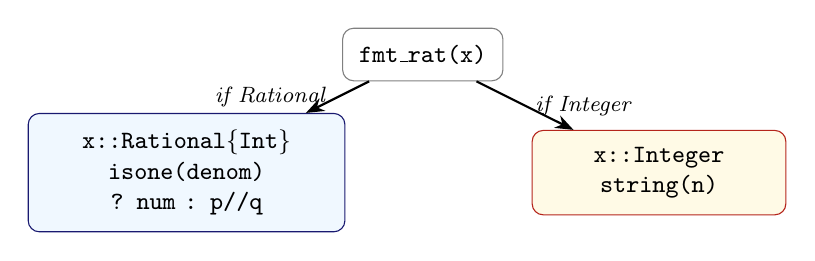
\begin{tikzpicture}[font=\small]
  \node[draw=gray, rounded corners, fill=white, inner sep=6pt]
    (call) at (0,0) {\cd{fmt\_rat(x)}};
  \node[draw=MidnightBlue, rounded corners, fill=examplebg, inner sep=6pt,
        text width=3.6cm, align=center]
    (rat) at (-3,-1.5) {\cd{x::Rational\{Int\}}\\
      \cd{isone(denom) ? num : p//q}};
  \node[draw=BrickRed, rounded corners, fill=notebg, inner sep=6pt,
        text width=2.8cm, align=center]
    (int) at (3,-1.5) {\cd{x::Integer}\\
      \cd{string(n)}};
  \draw[-Stealth, thick] (call) -- node[left, font=\footnotesize]{
    \textit{if Rational}} (rat);
  \draw[-Stealth, thick] (call) -- node[right, font=\footnotesize]{
    \textit{if Integer}} (int);
\end{tikzpicture}
\end{center}

\needspace{5\baselineskip}
\subsection{The \texttt{let} Closure Problem}

The \cd{let} fix in script~35 addresses one of the most
common bugs in reactive/callback-heavy code in any language:

\begin{center}
\begin{tabular}{p{6.5cm}p{6.5cm}}
\toprule
\textbf{Without \cd{let} (broken)} & \textbf{With \cd{let} (correct)} \\
\midrule
\begin{minipage}[t]{6.5cm}
\begin{minted}{julia}
for i in 1:3
  for d in 1:2
    on(tb.stored_string) do val
      # i and d are shared
      # captured by reference
      new_pts[i, d] = v  # WRONG
    end
  end
end
# After loop: i=3, d=2
# ALL callbacks update [3,2]
\end{minted}
\end{minipage}
&
\begin{minipage}[t]{6.5cm}
\begin{minted}{julia}
for i in 1:3
  for d in 1:2
    let row=i, col=d
      on(tb.stored_string) do val
        # row and col are local
        # captured by value
        new_pts[row, col] = v
      end
    end  # each callback has
  end    # its own row, col
end
\end{minted}
\end{minipage} \\
\bottomrule
\end{tabular}
\end{center}

\begin{insightbox}
\textbf{This pattern matters far beyond Julia.}
The same closure-capture bug exists in JavaScript
(\cd{var} in loops), Python (lambdas in loops),
and C\# (delegates in foreach).
The \cd{let} solution in Julia is the equivalent of
JavaScript's \cd{let} (block scope), Python's
default-argument trick, or C\#'s loop variable copy.
Once you understand it in one language, you recognise
it everywhere.
\end{insightbox}

\needspace{5\baselineskip}
\subsection{\texttt{Observable} vs \texttt{Ref}: Two Kinds of State}

Script~35 uses both, and the choice between them matters:

\begin{center}
\begin{tabular}{lp{4.5cm}p{4.5cm}}
\toprule
& \cd{Ref(x)} & \cd{Observable(x)} \\
\midrule
Read & \cd{ref[]} & \cd{obs[]} \\
Write & \cd{ref[] = v} & \cd{obs[] = v} \\
Notifies listeners? & No & Yes \\
Used for & \cd{active\_case}, \cd{switching},
  \cd{ax\_ref}, \cd{legend\_ref} &
  \cd{pts\_obs}, \cd{u\_obs},
  \cd{tog\_poly.active} \\
Callback? & None & \cd{on(obs) do ... end} \\
\bottomrule
\end{tabular}
\end{center}

The design rule: use \cd{Observable} when a change should
automatically trigger a redraw.
Use \cd{Ref} for internal bookkeeping state that does not
need to propagate.
\cd{switching} is a \cd{Ref} precisely because it is a
guard flag --- if it were an \cd{Observable}, setting it
could itself trigger the redraw you are trying to suppress.


% =============================================================
\needspace{8\baselineskip}
\section{Part 5: The Curvature Thread}
% =============================================================

\subsection{How Curvature Connects the Series}

Curvature is not introduced until script~34,
but the mathematical foundation is laid much earlier.
The thread runs from the polynomial derivatives in
scripts~01--05 all the way through to the live
$\kappa$ value in the script~35 equation panel.

\begin{center}
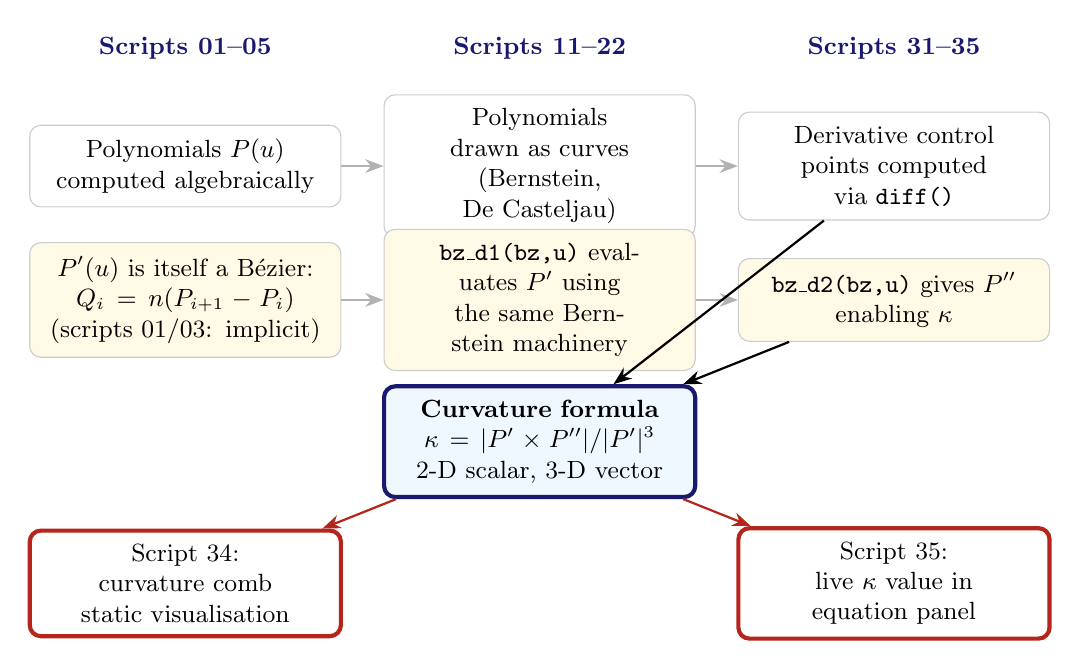
\begin{tikzpicture}[font=\small, node distance=0.4cm and 0.1cm]

  % Column headers
  \node[font=\bfseries\small, MidnightBlue] (h1) at (0,0)
    {Scripts 01--05};
  \node[font=\bfseries\small, MidnightBlue] (h2) at (4.5,0)
    {Scripts 11--22};
  \node[font=\bfseries\small, MidnightBlue] (h3) at (9,0)
    {Scripts 31--35};

  % Row 1
  \node[draw=gray!40, fill=white, rounded corners, inner sep=5pt,
        text width=3.6cm, align=center] (r1a) at (0,-1.5)
    {Polynomials $P(u)$ computed algebraically};
  \node[draw=gray!40, fill=white, rounded corners, inner sep=5pt,
        text width=3.6cm, align=center] (r1b) at (4.5,-1.5)
    {Polynomials drawn as curves\\ (Bernstein, De Casteljau)};
  \node[draw=gray!40, fill=white, rounded corners, inner sep=5pt,
        text width=3.6cm, align=center] (r1c) at (9,-1.5)
    {Derivative control points computed\\ via \cd{diff()}};

  % Row 2
  \node[draw=gray!40, fill=notebg, rounded corners, inner sep=5pt,
        text width=3.6cm, align=center] (r2a) at (0,-3.2)
    {$P'(u)$ is itself a B\'{e}zier:\\ $Q_i = n(P_{i+1}-P_i)$\\
     (scripts 01/03: implicit)};
  \node[draw=gray!40, fill=notebg, rounded corners, inner sep=5pt,
        text width=3.6cm, align=center] (r2b) at (4.5,-3.2)
    {\cd{bz\_d1(bz,u)} evaluates $P'$ using\\ the same Bernstein machinery};
  \node[draw=gray!40, fill=notebg, rounded corners, inner sep=5pt,
        text width=3.6cm, align=center] (r2c) at (9,-3.2)
    {\cd{bz\_d2(bz,u)} gives $P''$\\ enabling $\kappa$};

  % Row 3
  \node[draw=MidnightBlue, fill=examplebg, rounded corners,
        inner sep=5pt, text width=3.6cm, align=center,
        line width=1.5pt] (r3) at (4.5,-5.0)
    {\textbf{Curvature formula}\\ $\kappa = |P'\times P''| / |P'|^3$\\
     2-D scalar, 3-D vector};

  % Row 4
  \node[draw=BrickRed, fill=white, rounded corners,
        inner sep=5pt, text width=3.6cm, align=center,
        line width=1.5pt] (r4a) at (0,-6.8)
    {Script 34:\\ curvature comb\\ static visualisation};
  \node[draw=BrickRed, fill=white, rounded corners,
        inner sep=5pt, text width=3.6cm, align=center,
        line width=1.5pt] (r4b) at (9,-6.8)
    {Script 35:\\ live $\kappa$ value in\\ equation panel};

  \draw[-Stealth, thick, gray!60] (r1a) -- (r1b);
  \draw[-Stealth, thick, gray!60] (r1b) -- (r1c);
  \draw[-Stealth, thick, gray!60] (r2a) -- (r2b);
  \draw[-Stealth, thick, gray!60] (r2b) -- (r2c);
  \draw[-Stealth, thick] (r1c) -- (r3);
  \draw[-Stealth, thick] (r2c) -- (r3);
  \draw[-Stealth, thick, BrickRed] (r3) -- (r4a);
  \draw[-Stealth, thick, BrickRed] (r3) -- (r4b);

\end{tikzpicture}
\end{center}

\needspace{5\baselineskip}
\subsection{The Derivative Control Point Insight}

The key insight that makes efficient curvature computation
possible is that the derivative of a B\'ezier curve is
itself a B\'ezier curve.
This means \cd{eval\_poly} --- the same function that
evaluates the original curve --- can also evaluate the
derivative and second derivative.
No symbolic differentiation is needed.

\begin{minted}{julia}
# All three use the same evaluator:
bz_point = eval_poly(bz.points,  u)   # P(u)
bz_d1    = eval_poly(bz.d1_pts,  u)   # P'(u)
bz_d2    = eval_poly(bz.d2_pts,  u)   # P''(u)
\end{minted}

\begin{center}
\begin{tabular}{llll}
\toprule
Quantity & Control points & Degree & Result \\
\midrule
$P(u)$ & \cd{bz.points} ($n\times d$) & $n-1$ &
  Point on curve \\
$P'(u)$ & \cd{bz.d1\_pts} ($(n-1)\times d$) & $n-2$ &
  Tangent vector \\
$P''(u)$ & \cd{bz.d2\_pts} ($(n-2)\times d$) & $n-3$ &
  Curvature direction \\
\bottomrule
\end{tabular}
\end{center}

\needspace{5\baselineskip}
\subsection{2-D vs 3-D Curvature: One Formula, Two Implementations}

The curvature formula $\kappa = |P' \times P''| / |P'|^3$
is the same in both dimensions, but the cross product
means different things:

\begin{center}
\begin{tabular}{p{2.5cm}p{5cm}p{4.5cm}}
\toprule
Dimension & Cross product $P' \times P''$ & Code \\
\midrule
2-D &
  Scalar: $P'_x P''_y - P'_y P''_x$\\
  (the $z$-component of the 3-D cross product) &
  \cd{abs(d1[1]*d2[2] - d1[2]*d2[1])} \\[6pt]
3-D &
  Vector of length $|P'||P''|\sin\theta$ &
  \cd{norm(cross(d1, d2))} \\
\bottomrule
\end{tabular}
\end{center}

The 2-D formula avoids the overhead of constructing a
zero-padded 3-D vector just to call \cd{cross}.
The 3-D formula reuses the \cd{LinearAlgebra.cross}
function directly.

\needspace{5\baselineskip}
\subsection{The Curvature Comb as a Design Verification Tool}

Beyond being visually striking, the curvature comb in
scripts~34--35 serves a practical purpose in curve design.

\begin{insightbox}
\textbf{What designers read from a curvature comb:}

\textbf{Uniform comb} (constant spike height) ---
the curve has constant curvature.
A circle has a perfectly flat comb envelope.

\textbf{Smooth comb} (continuously varying height) ---
curvature changes gradually.
This is desirable for fair curves in industrial design.

\textbf{Spiky or discontinuous comb} ---
curvature changes abruptly.
At a kink (discontinuous tangent), the comb has a
spike of infinite height.
This is undesirable in automotive body panels, aerofoils,
and other applications where visual smoothness matters.

The quadratic B\'ezier in Case~1 produces a smooth,
symmetric comb --- confirming it is a fair curve.
The quartic B\'ezier in Case~2 shows a more complex
profile reflecting the tighter bends introduced by the
off-axis control points $P_1$ and $P_2$.
\end{insightbox}


% =============================================================
\needspace{8\baselineskip}
\section{Summary: What the Series Teaches About Software Design}
% =============================================================

Looking at the 15 scripts together, five software design
principles emerge:

\begin{center}
\renewcommand{\arraystretch}{1.4}
\begin{tabular}{lp{5cm}p{5cm}}
\toprule
Principle & How it appears & Scripts \\
\midrule
\textbf{Separation of concerns} &
  Math, drawing, and UI are separate functions
  (\cd{bz\_point}, \cd{draw\_all!}, \cd{redraw}) &
  31--35 \\[4pt]
\textbf{Single point of change} &
  \cd{const CASE = N} controls everything &
  01--05, 31--34 \\[4pt]
\textbf{Generalise at the right time} &
  Quadratic first, then quartic, then generic ---
  not generic from the start &
  11$\to$21$\to$31 \\[4pt]
\textbf{Reuse by composition} &
  \cd{draw\_all!} is called by both \cd{draw\_and\_show}
  (scripts 34) and \cd{redraw} (script 35) &
  34--35 \\[4pt]
\textbf{Fail safely} &
  \cd{tryparse}, \cd{isnothing} guards,
  \cd{speed < 1e-10 \&\& return 0.0} &
  34--35 \\
\bottomrule
\end{tabular}
\end{center}

\vspace{2em}\hrule\vspace{0.5em}
{\small\textcolor{gray}{%
Code analysis for the B\'ezier series, scripts 01--35
\textbar{} Directed and curated by E.R.\ Nurwijayadi
\textbar{} Code and explanations AI-generated}}

\end{document}
